\chapter{QASM: Question and Answer Social Media}
\doublespacing
\label{chap:qasm}
\minitoc

\section{Introduction: formalizing and linking knowledge on Q\&A sites}
Community Question Answering (CQA) services provide a platform where users can ask expert for help. Since questions and answers can be viewed and searched afterwards, people with similar questions can also directly find solutions by browsing this content. Therefore, effectively managing these content is a key issue. 

In order to using semantic web technology, there are two basic steps, formalizing and linking. The first one is to formalize unstructured data into structure data using domain ontology. This chapter is focus on this step. The second one is to link to open knowledge base. We introduce this step in Chapter \ref{chap:label}

We think that there are two kinds of information in our scenario. The first one is original user-generated content, for instance, question answer contents. Another one is latent information extracted by data mining techniques, for instance, community and temporal information. It is important to formalize both of them. SIOC ontology is the most popular vocabulary to formalize online community, but it does not support to formalize the latent information extracted by data mining techniques. 

In this chapter, we describe QASM (Question \& Answer Social Media), a prototype system based on social media mining and semantic web technology to manage the two main resources in the CQA sites: users and contents. We present the QASM vocabulary used to formalize both the two kinds of information. Then we briefly introduce our method to extract these latent knowledge from the CQA sites.


\section{QASM System Description: managing explicit and implicit knowledge}
\subsection{Overview: combine social media mining and semantic web}
Figure \ref{fig:overview} presents an overview of QASM. We first use the SIOC ontology\footnote{http://sioc-project.org/ontology} to construct an RDF dataset from social media data extracted from a CQA site:StackOverflow. Then we use social media mining techniques to extract topics, interests and expertise levels , temporal dyanmics from this dataset. We formalize them with the QASM vocabulary and enrich our RDF dataset with these latent information. As a result, we provide an integrated and enriched Q\&A triple store which contains both user interests, user expertise, user temporal dynamics and topics. Finally, we linked our dataset with DBpedia and use the extra knowledge to generate labels for topics. Based on the QASM RDF dataset, we can provide the users of the Q\&A site with several services to find relevant experts for a question and to search for similar questions.

\begin{figure}%[htbp]
\centering
%\epsfig{file=fly.eps, height=1in, width=1in} % use this if you use "pdflatex"
%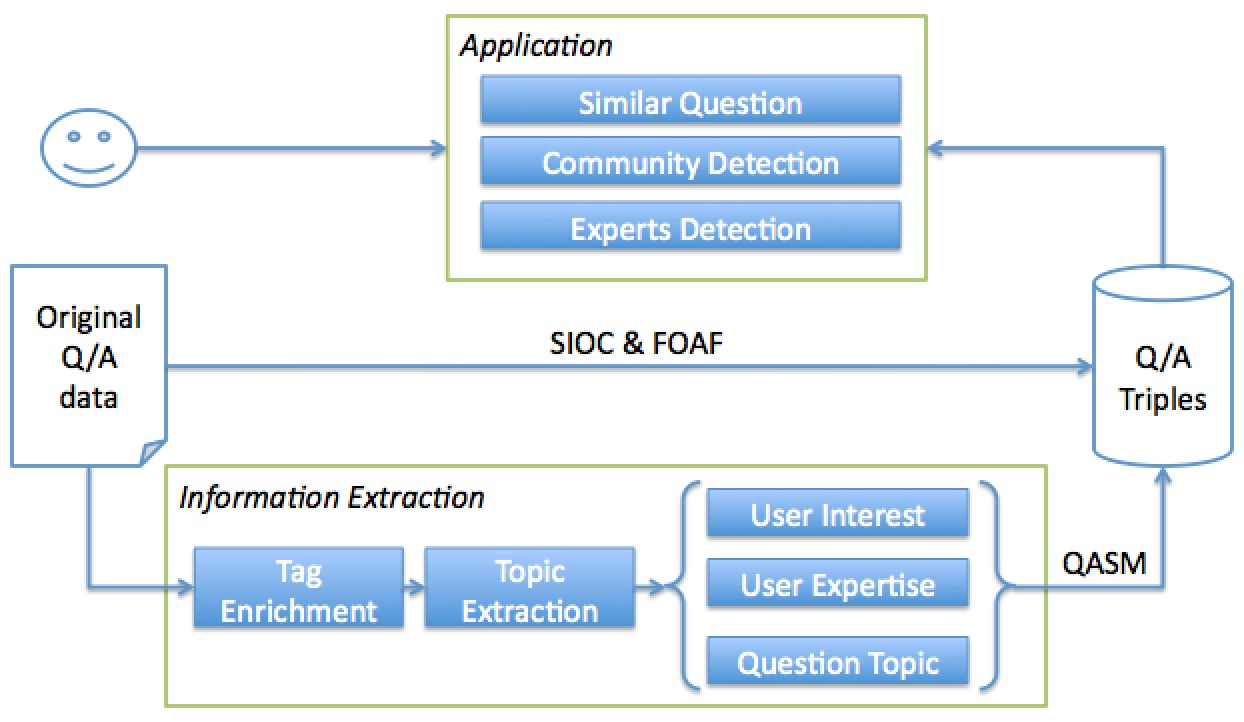
\includegraphics[height=1.857in, width=3.2in]{overview.png}  
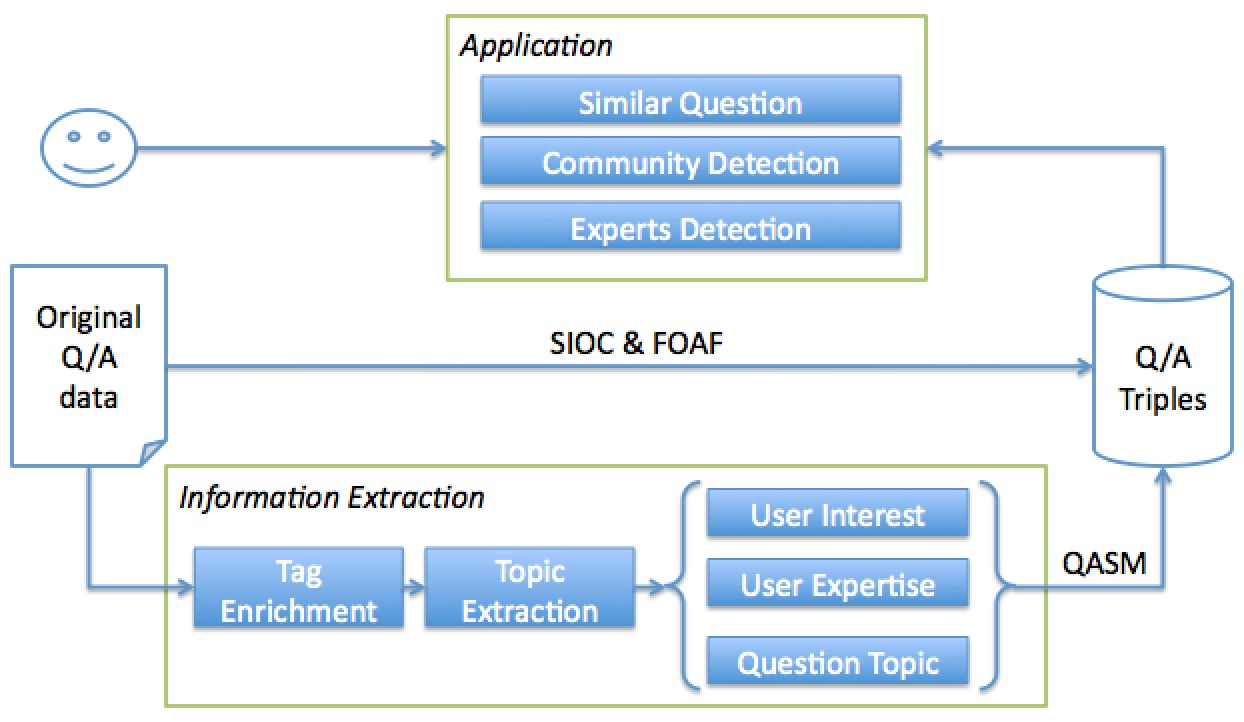
\includegraphics[width=3.2in]{overview.png}  
\caption{Overview of QASM}
\label{fig:overview} 
\end{figure}

\subsection{QASM Vocabulary: formalize Q\&A information}
\begin{figure}[htbp]
\centering
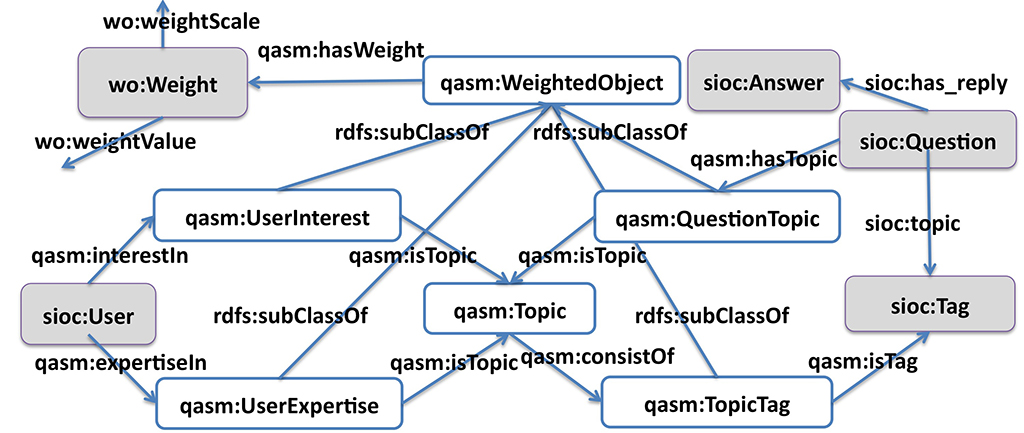
\includegraphics[width=3.7in]{ontologyv2.jpg}  
\caption{Overview of the QASM vocabulary}
\label{fig:coreontology} 
\end{figure}

From the overview, there are mainly two kinds of information to formalize. Part of them are explicit, which is the original user-generated content, such as Q\&A contents, user profile, votes, and timestamps. Part of them are implicit, which is detected by social media mining techniques, such as user interest, overlapping communities, user expertise, user activities. 

Existing work mainly focus on how to formalize the explicit part. We are focusing on extending existing work by formalizing the implicit part. Thus, we proposed QASM vocabulary. Figure \ref{fig:coreontology} provides an overview of our ontology. It reuses both the SIOC ontology and the Weighting ontology\footnote{http://smiy.sourceforge.net/wo/spec/weightingontology.html}.
The QASM vocabulary\footnote{It is available online at http://ns.inria.fr/qasm/qasm.html} enables to model both explicit and implicit information from Q\&A sites. Table \ref{tab:qaontoclass}shows the main classes used in our work.


\begin{sidewaystable}
    \centering
    \begin{tabular}{c|c|c|c}
    \hline
    Class &  Description & type & onto \\ \hline
    User  & active user & explicit &  sioc:User \\ \hline
    Question & questions post & explicit & sioc:Question \\ \hline
    Answer  & answer post & explicit & sioc:Answer \\ \hline
    Tag & tags used to label questions & explicit & sioc:Tag \\ \hline
    Word & words used in Q\&A content & explicit & qasm:Word \\ \hline
    Topic & bag of words/tags & implicit & QASM:Topic \\ \hline     
    UserInterest& User interest over topic distribution & implicit& qasm:UserInterest\\ \hline
    UserExpertise & User expertise over topic distribution &implicit& qasm:UserExpertise \\ \hline
    TopicTag &Topic over tags distribution&implicit &qasm:TopicTag \\ \hline
    
    TopicWord&Topic over words distribution &implicit & qasm:TopicWrod\\ \hline
    
    UserActivity&Topic over users distribution & implicit &qasm:UserActivity \\ \hline
    
    TopicTrend &Topic over time distribution &implicit & qasm:TopicTrend\\ \hline
          
    \end{tabular}
    \caption{the Vocabulary (class) used in our work}
    \label{tab:qaontoclass}
\end{sidewaystable}


\begin{sidewaystable}
    \centering
    \begin{tabular}{c|c|c|c|}
    \hline
        Property &  Description & from & to  \\ 
    \hline
    qasm:interestIn  & a user is interested in a topic & sioc:User &  qasm:UserInterest \\ \hline
    qasm:isTopic     & a userInterest object associate with a topic &qasm:UserInterest  &qasm:Topic \\ \hline
    qasm:hasWeight   & a userInterest object associate with a weight&qasm:UserInterest  &wo:Weight \\ \hline
    
    qasm:expertiseIn & a user has expertise in a topic & sioc:User & qasm:UserExpertise \\ \hline
    qasm:isTopic     & a userExpertise object associate with a topic &qasm:UserExpertise &qasm:Topic \\ \hline
    qasm:hasWeight   & a userExpertise object associate with a weight &qasm:UserExpertise &wo:Weight \\ \hline
    
    qasm:consistOf   & a topic is consist of tags   &qasm:Topic &qasm:TopicTag \\ \hline
    qasm:isTag     & a topic tag object associate with a tag  &qasm:TopicTag &sioc:Tag \\ \hline
    qasm:hasWeight   & a topic tag object associate with a weight &qasm:TopicTag &wo:Weight \\ \hline
    
    qasm:consistOf   & a topic is consist of words  &qasm:Topic &sioc:TopicWord \\ \hline
    qasm:isWord     & a topic word object associate with a word  &qasm:TopicWord &sioc:Word \\ \hline
    qasm:hasWeight   & a topic word object associate with a weight &qasm:TopicTag &wo:Weight \\ \hline
    
    qasm:isPopularAt  & a topic is popular at a time point & qasm:Topic &  qasm:TopicYearTrend \\ \hline
    qasm:isYear     & a topic trend object associate with a time point &qasm:TopicYearTrend  &qasm:Year \\ \hline
    qasm:hasWeight   & a topic trend object associate with a weight&qasm:TopicYearTrend  &wo:Weight \\ \hline
    
    qasm:hasActiveUser & a topic has an active user & qasm:Topic &  qasm:UserActivity \\ \hline
    qasm:isUser     & a user activity object associate with a user &qasm:UserActivity  &sioc:User \\ \hline
    qasm:hasWeight   & a user activity object associate with a weight&qasm:UserActivity  &wo:Weight \\ \hline

          
    \end{tabular}
    \caption{the Vocabulary (property) used in our work}
    \label{tab:qaontoproper}
\end{sidewaystable}

Table \ref{tab:qaontoproper} shows several proprieties used in our work. Since our work mainly generate distributions, we use the same patter to formalize these distributions. As an example, we show an example of formalizing a distribution in Figure \ref{fig:chp3ontoexample}. 

\begin{figure}%[htbp]
\centering
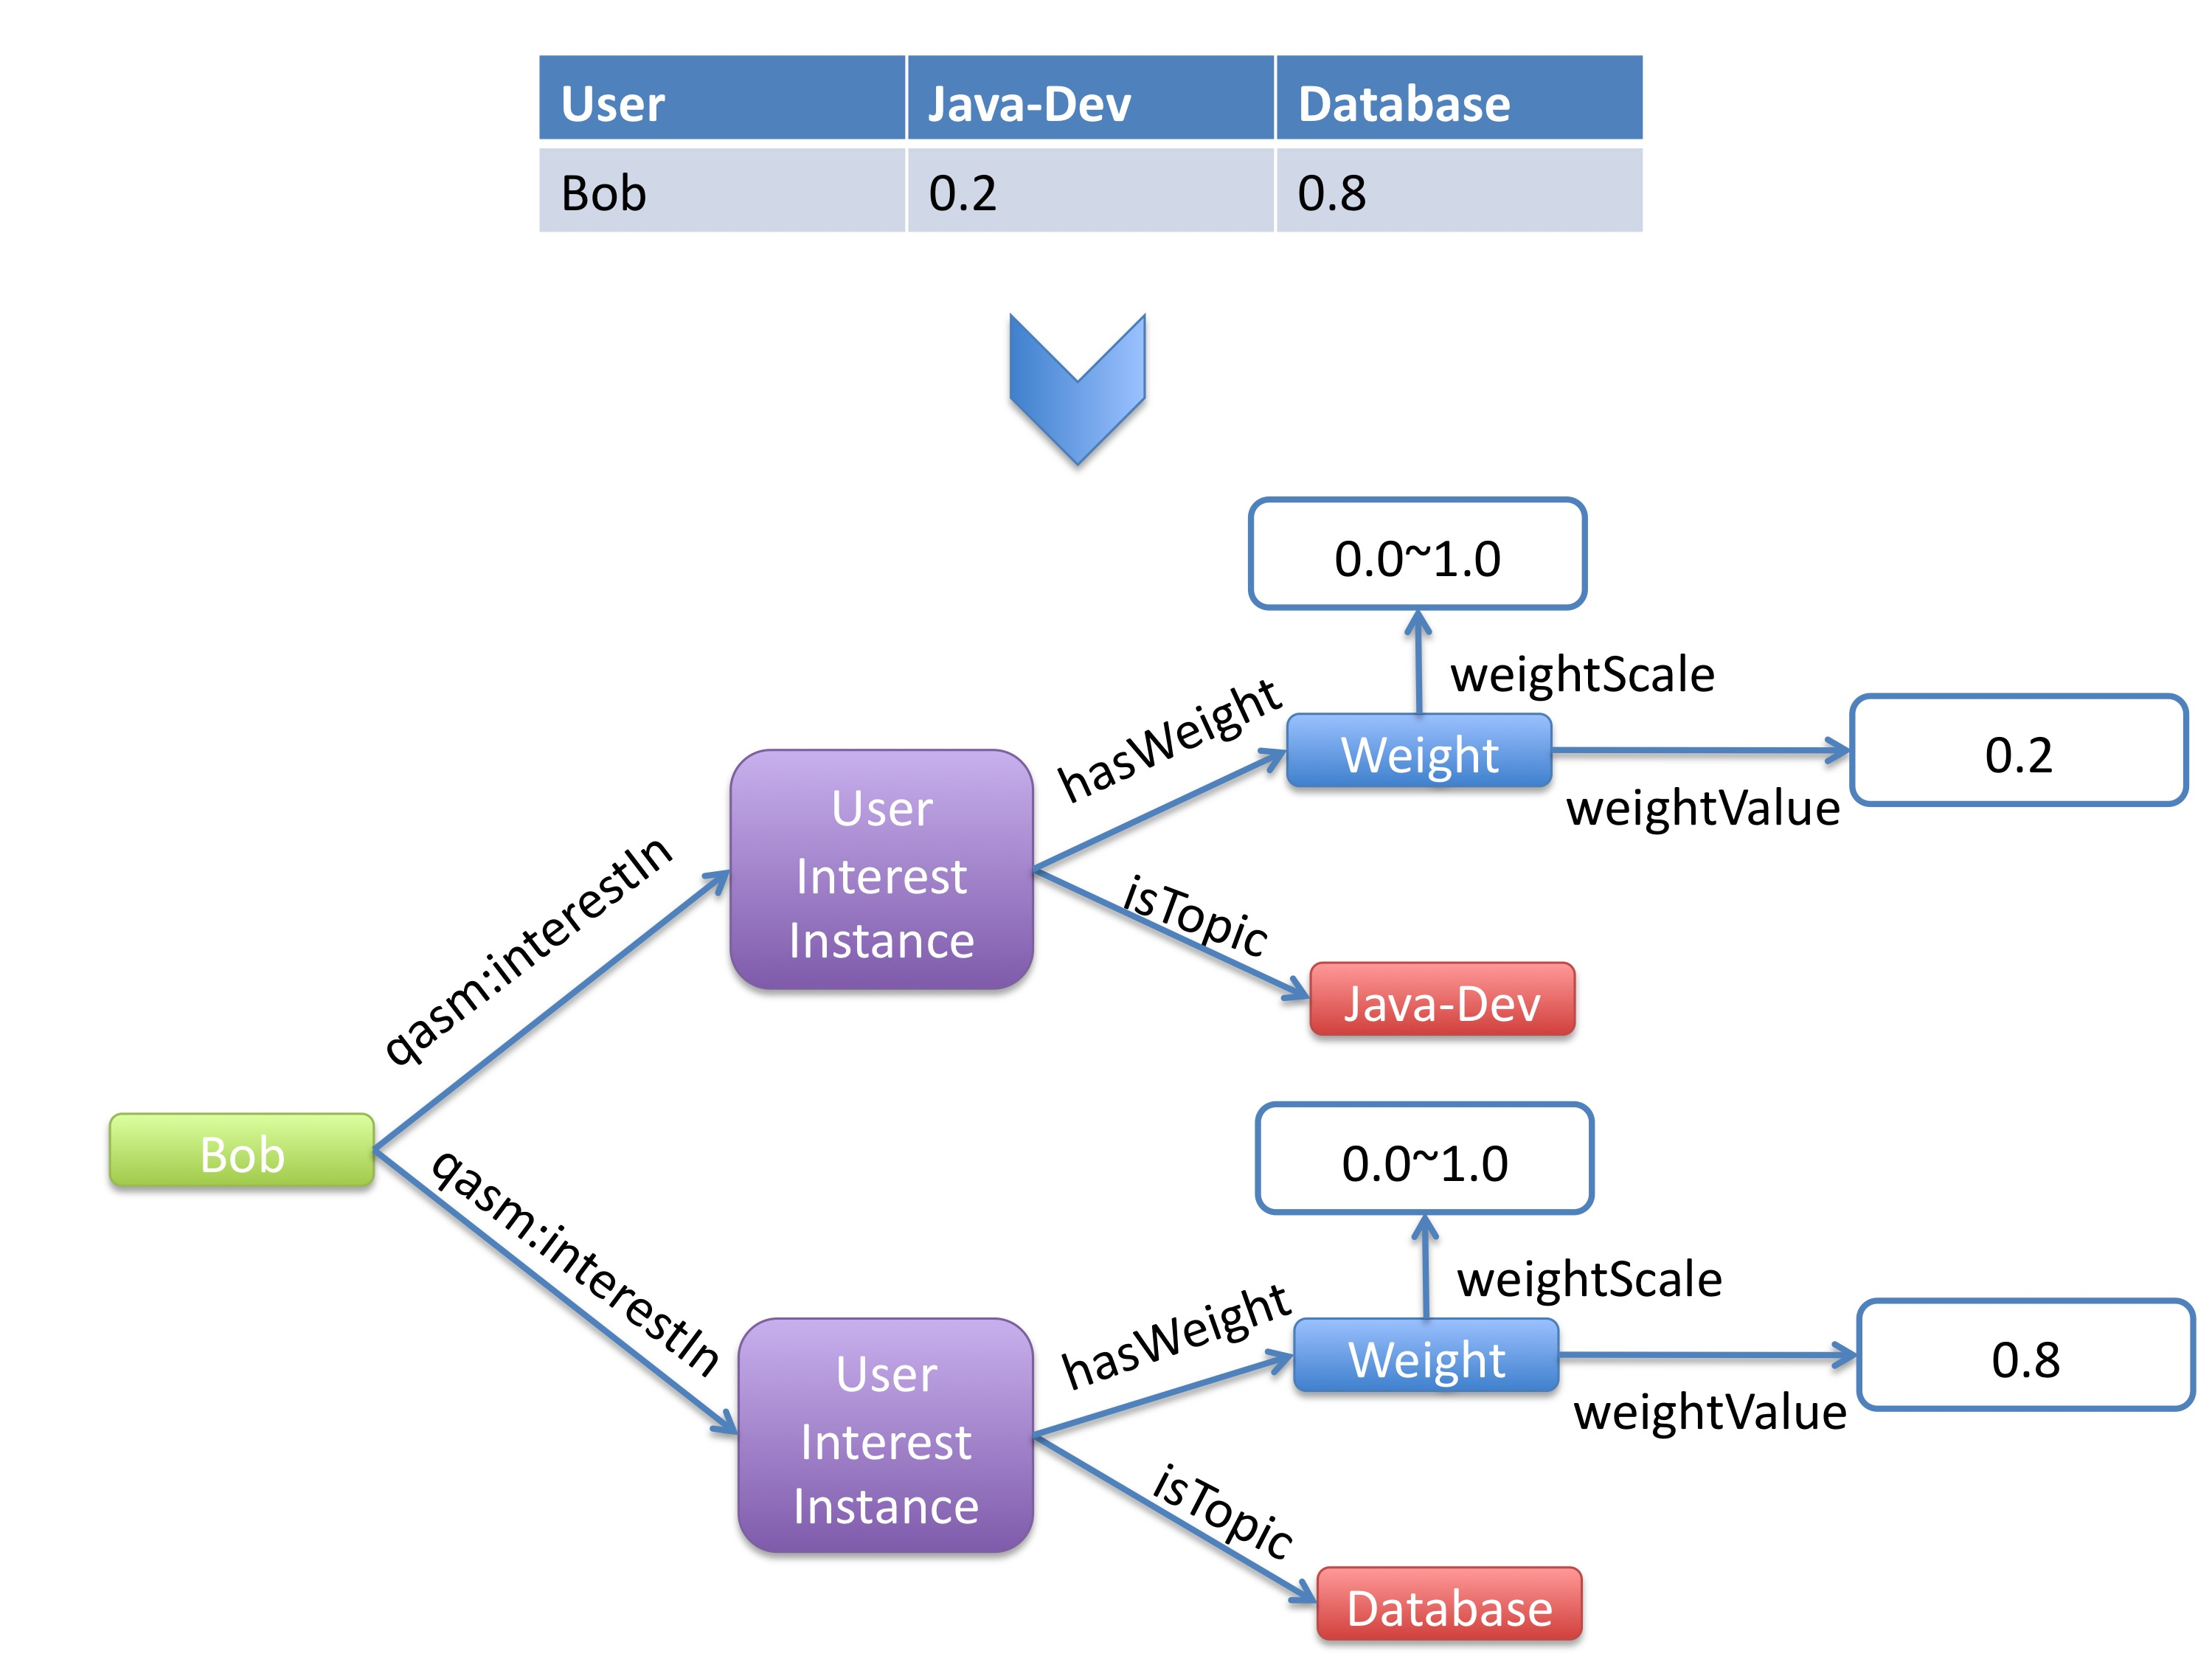
\includegraphics[width=3.2in]{chp3ontoExample.jpg}  
\caption{An example of formalize a distribution}
\label{fig:chp3ontoexample} 
\end{figure}

We explain some core classes and properties as below.

\begin{itemize}
\item \texttt{qasm:Topic} represents a set of tags/words related to a specified topic.
In our models, tags/words belong to instances of \texttt{qasm:Topic}, we also consider different tags/words have different weights for each topic.
\item \texttt{qasm:WeightedObject} is used to describe the weight that a specified subject has with regard to a specified object. This class has four subclasses which represent question topics, users' interests, users' expertise and tag topics respectively. In fact, this class is used to model the distributions we extracted from the original data. For example, topic-tag distribution, user-interest distribution.
\item \texttt{qasm:interestIn} is used to describe the user-interest distribution. This property is different from \texttt{foaf:interest} for its range. In FOAF people are interested in documents, while in QASM a user is interested in a topic to a certain degree (a weight).
\item \texttt{qasm:expertiseIn} is used to describe the user-expertise distribution. A user has different weights for different topics.
\item \texttt{qasm:isPopularAt} is used to describe the topic-time distribution. A topic has different popularity at different time point.
\item \texttt{qasm:hasActiveUser} is used to describe the topic-user distribution. Different users perform different activities on a topic.
\end{itemize}



\subsection{Social media mining: extract the latent knowledge}

Topics, interests, expertise, activity, trend are implicit information in the available raw CQA data. We use social media mining techniques to extract this knowledge.
In Chapter \ref{chap:ttd}, we propose a Tag Tree Distribution method to efficiently extract topic from tags while preserving good quality. Besides, in Chapter \ref{chap:ttea}, we jointly model topic, interest, expertise and trend to extract the relations between them, such as user-topic, topic-time, user-expertise, user-interest etc. In addtion, Chapter \ref{chap:label} propose a method by using DBpedia to generate label for a bag of words which is used to define a topic. 
We list all the descriptions, examples of the latent knowledge extracted by our models. We also list the related vocabulary for each of them.


\textbf{Topic}: A bag of words or tags which are closely related. Words are the content of questions or answers, tags are attached to questions. For example, the topic-tag distribution \textit{Database}:\{{\textit{mysql}: 0.5, \textit{sql}: 0.3, \textit{query}: 0.2\}. expresses that topic \textit{Database} is related to tags \textit{mysql}, \textit{sql}, and \textit{query}. We use \texttt{qasm:TopicTag} and \texttt{qasm:TopicWord} to formalize this distribution.

\textbf{User Topical Interest}: A user is interested in different topics with different levels. For example, the user-topic distribution \textit{Alice}:\{{\textit{Database}: 0.8, \textit{Java}: 0.2\} expresses that \textit{Alice} prefers to answer questions related to \textit{Database}, but rather not about \textit{Java}. We use \texttt{qasm:UserInterest} to formalize this distribution.

\textbf{User Topical Activity}:  Different users are interested in the same topic with different levels. For example, the topic-user distribution \textit{Database}:\{{\textit{Alice}: 0.8, \textit{Bob}: 0.2\} expresses that \textit{Alice} prefers to answer question related to \textit{Database}, while \textit{Bob} is not willing to contribute answers to it. We use \texttt{qasm:UserActivity} to formalize this distribution.

\textbf{Topic Trend}: A topic is popular at different points in time with different levels. For example,the topic-time distribution \textit{Database}:\{{\textit{May/2013}: 0.2, \textit{June/2013}: 0.3, \textit{July/2013}: 0.5\} expresses that the topic \textit{Database} is increasingly popular.% while the topic \textit{java} remains stable. 
We use \texttt{qasm:TopicTrend} to formalize this distribution.


\textbf{User Topical Expertise}: A user has expertise in different topics with different levels. For example, the topic-expertise distribution for \textit{Alice} \textit{ios}:\{{\textit{High}: 0.2, \textit{Medium}: 0.7, \textit{Low}: 0.1\} expresses that \textit{Alice}'s expertise on topic \textit{ios} is probably in medium level. We use \texttt{qasm:UserExpertise} to formalize this distribution.


\section{Summary: an effective way to manage q\&a sites}
\label{sec:future}
We presented QASM, a Q\&A system combining social media mining and semantic web models and technologies to manage Q\&A users and content in CQA sites. This chapter provide us a framework to manage user-generated content and extracted latent knowledge on Q\&A sites. In the next chapters, we will focus on how to efficiently extract these latent knowledge, such as topics and communities. And how to extract more latent information such as topic based temporal dynamics, topic based expertise.





